\documentclass[12pt]{article}
\usepackage{ctex}
\usepackage{graphicx}
\usepackage{indentfirst}
\usepackage{amsmath}
\usepackage{float}
\usepackage{amssymb}
\usepackage{bm}
\title{第六周作业报告}
\author{佐藤拓未 20300186002}
\date{}

\begin{document}
	
	\maketitle
	
	\begin{center}
		\textbf{第一问}
	\end{center}



\noindent 用Newton表示重新写出Adams格式.\\


\noindent \textbf{解:}不妨只考虑多步Adams-Moulton格式, 首先对$t_{n+1-k}, ..., t_n, t_{n+1}$共$k+1$个节点作关于$f_{n+1-k}, ..., f_n, f_{n+1}$的Newton途径$k$次插值多项式
$$P_k(t)=f_{n+1-k}+   f[t_{n+1-k},t_{n+2-k}](t-t_{n+1-k})+\cdots+f[t_{n+1-k},\cdots,t_n,t_{n+1}](t-t_{n+1-k})\cdots(t-t_n)$$
那么可以导出线性多步格式
\begin{align*}
	u_{n+1}-u_n&=\int_{t_n}^{t_{n+1}}P_k(t){\rm d} t\\
	&=\Delta{t}f_{n+1-k}+f[t_{n+1-k},t_{n+2-k}]\int_{t_n}^{t_{n+1}}(t-t_{n+1-k}){\rm d}t+\cdots\\
	&\quad+f[t_{n+1-k},\cdots,t_n,t_{n+1}]\int_{t_n}^{t_{n+1}}(t-t_{n+1-k})\cdots(t-t_n){\rm d} t
\end{align*}

\noindent 考虑差分$\Delta^0f_{n}=f_{n}$, $\Delta^{j+1}f_n=\Delta^jf_{n+1}-\Delta^jf_{n}$以及$\Delta^sf_n=s!\Delta{t}^sf[x_n,x_{n+1},\cdots,x_{n+s}]$, 那么多步格式可以简记为
$$u_{n+1}-u_n=\Delta{t}\sum_{s=0}^{k}\frac{\Delta^s f_{n+1-k}}{s!\Delta{t}^{s+1}}\int_{t_n}^{t_{n+1}}\phi_s(t){\rm d}t$$
\noindent 其中$\phi_s(t)$是$s$次多项式

\begin{align*}
	\phi_s(t)=\begin{cases}
		(t-t_{n+1-k})\cdots(t-t_{n+s-k}) \quad \quad & s=2,3,\cdots,k\\
		1 &s=0
	\end{cases}
\end{align*}

\noindent 更进一步, 作变换$t=t_n+\tau \Delta{t}$, 那么$$\int_{t_n}^{t_{n+1}}\phi_s(t){\rm d}t=\Delta{t}^{s+1}\int_{0}^{1}\prod_{i=1}^{s}(\tau+k-i){\rm d}\tau$$
\noindent 从而多步格式为$$u_{n+1}-u_n=\Delta{t}[f_{n+1-k}+\sum_{s=1}^{k}\frac{\Delta^s f_{n+1-k}}{s!}\int_{0}^{1}\prod_{i=1}^{s}(\tau+k-i){\rm d}\tau]$$
\noindent 类似地, 若考虑$\nabla^0f_n=f_n, \nabla^{j+1}f_n=\nabla^jf_n-\nabla^jf_{n-1}$, 则多步格式也可以写为
$$u_{n+1}-u_n=\Delta{t}[f_{n+1}+   \sum_{s=1}^{k}\frac{\nabla^sf_{n+1}}{s!}\int_{0}^{1}\prod_{i=1}^{s}(\tau+i-2){\rm d}\tau]$$
\\
\begin{center}
	\textbf{第二问}
\end{center}
	
\noindent 在用Adams格式和Gear格式时, 需要给定初始$k$步值, 请对标准测试问题, 用四阶的Adams格式和四阶的Gear格式, 观察不同的初始选取对精度的影响: 1) 用精确的初始值; 2) 用显式Euler格式计算初始的$k-1$个值; 3) 用二至四阶Runge-Kutta格式计算初始的$k-1$个值.\\
\\
\textbf{解:}欲从两个角度分析精度: 1) 不同的初值对相同的格式收敛精度影响; 2) 当初值相同时, 不同迭代格式对收敛精度的影响.\\
对于标准测试问题$\frac{{\rm d}u}{{\rm d}t}=au$, 取$a=-2, u_0=1, t_0=0, T=1, \Delta{t}=2^{-i}, N=[\frac{T}{\Delta{t}}]$, 并令$i$变动以观察收敛阶.\\
由于A-M四阶方法是三步格式, 因此只需要$3$个初值, 但是需要多求解一个非线性方程; 由于A-B与GEAR四阶方法都是四步格式, 因此它们需要$4$个初值, 但不需要求解非线性方程.\\
\textbf{1) 不同的初值对相同的格式收敛精度影响: }\\
首先, 如果初值是精确的: $\forall i=1,2,\cdots$, $\Delta{t}=2^{-i}$确定, 我们可以考虑不同格式的末项相对误差. $u_{N}$为给定格式的末项, 则有末项与精确解的相对误差$$\vert \epsilon_N \vert=\frac{\vert u(T)-u_N\vert}{\vert u(T)\vert}$$
\noindent 若格式是$p$阶格式, 还有
\begin{align*}
	\vert \epsilon_N \vert &= O(\Delta{t}^p)\overset{\triangle}{=}C\Delta{t}^p\\
	\ln \vert \epsilon_N \vert \ &= \ln C + p\ln\Delta{t}=\ln C - ip\ln2
\end{align*}
\noindent 从而末项相对误差的对数值与$i$是线性关系.\\
若初值是不精确的: 还需要考虑初值带来的影响, 从而即便格式相同, 但当初值有扰动时, 它们的收敛精度也会不一样.\\
事实上, A-M和A-B格式满足根条件: 即它们的第一特征多项式$\lambda -1 $的根落在单位圆盘, 从而可知它们具有稳定性; 另外, 两个四阶格式都是相容的, 从而具有以下收敛性估计:$$\vert  \epsilon_N\vert \le C_1\vert \vert \bm{\epsilon_{k-1}}\vert \vert+C_2\Delta{t}^p$$
\noindent 从而由上面的估计,可知初值的误差也会改变收敛精度.\\
\noindent 当考虑的是A-M四阶格式时, 收敛精度最差的是显式Euler初值下的收敛精度; 收敛精度最好的是精确初值与Kutta四阶初值下的收敛精度, 具体见图1. \\
当考虑的是A-B四阶格式时, 收敛精度最差的还是显示Euler初值下的收敛精度; 而此时精确初值与Kutta三至四阶初值下的收敛精度是相当接近的, 具体见图2.


\begin{figure}[H]
	\centering
	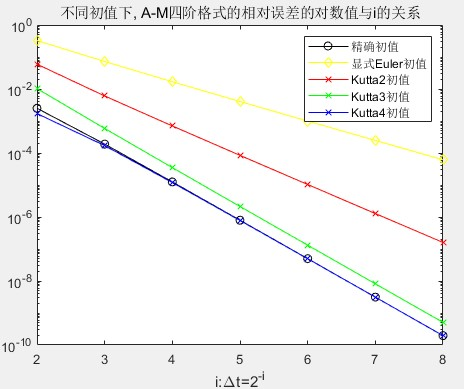
\includegraphics[width=0.7\textwidth]{1}
	\caption{A-M四阶格式在不同初值下的收敛阶}
\end{figure}
\begin{figure}[H]
	\centering
	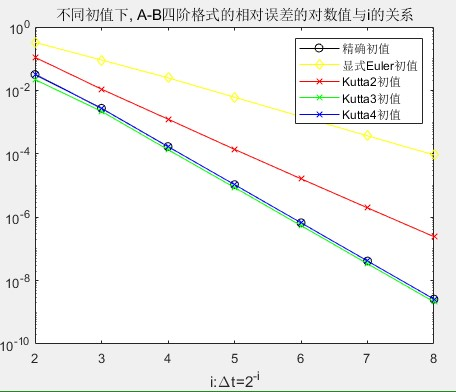
\includegraphics[width=0.7\textwidth]{2}
	\caption{A-B四阶格式在不同初值下的收敛阶}
\end{figure}
\begin{figure}[H]
	\centering
	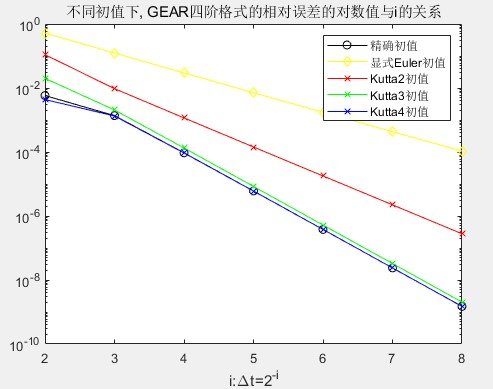
\includegraphics[width=0.7\textwidth]{3}
	\caption{Gear四阶格式在不同初值下的收敛阶}
\end{figure}
\noindent 当格式为四阶Gear格式时, 不同初值下的收敛精度与A-B四阶格式类似, 具体见上图.\\
总的来说, 通过Euler显格式求得的初值与精确初值相差较多, 从而导致了在三个不同四阶格式中的精度表现并不好; 通过Kutta二阶方法求得的初值在精度上是不如精确初值与Kutta三至四阶方法求得的初值, 从而使得在Kutta二阶初值下, 三者的收敛精度不如后者; 而Kutta三至四阶初值相对来说比较靠近精确初值, 从而初值的扰动对收敛阶的影响是较小的.\\
\quad \\

\noindent \textbf{2) 当初值相同时, 不同迭代格式对收敛精度的影响: }\\
\underline{精确初值:}\\
当初值是精确的, 三个不同四阶方法的收敛阶只取决于它们的相容性, 即三者的收敛阶均为四阶. 从图4中就可看出, 它们的斜率都是相同的.
\begin{figure}[H]
	\centering
	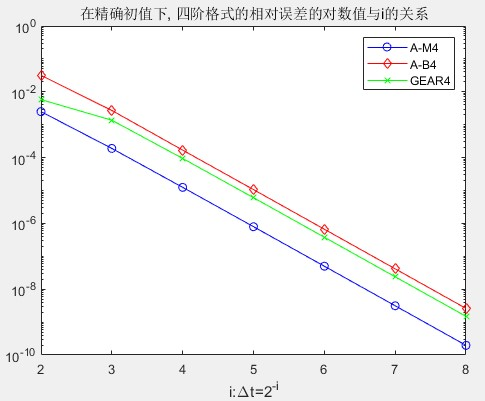
\includegraphics[width=0.7\textwidth]{4}
	\caption{精确初值}
\end{figure}
\noindent \underline{显式Euler初值:}\\
从图5中可以看出, 显式Euler初值下, 它们的收敛阶是相同的, 然而它们总体的收敛阶较差: 相较于精确初值下, 三种不同格式的相对误差在$i=8$时被控制在$10^{-8}$以内, 但在显式Euler初值下, 只能被控制在$1.07\times10^{-4}$以内.\\
\noindent \underline{Kutta初值:}\\
由图6、7、8可知, 在Kutta初值下, 三个不同的四阶格式最终的末项相对误差会随着Kutta方法的阶数提高而降低, 这是因为当Kutta的$p$阶格式的精度会随着$p$增高而提升, 从而使近似初值与精确初值越来越靠近. 在数值上, Kutta二阶初值下, 三者的精度最终在$10^{-7}$与$10^{-6}$之间; Kutta三阶至四阶初值下, 最终精度均被控制在$10^{-8}$.

\begin{figure}[H]
	\centering
	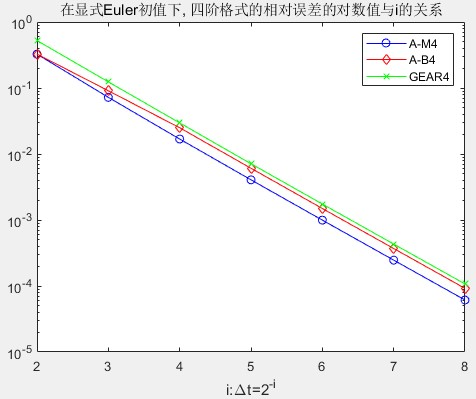
\includegraphics[width=0.7\textwidth]{5}
	\caption{显式Euler初值}
\end{figure}
\begin{figure}[H]
	\centering
	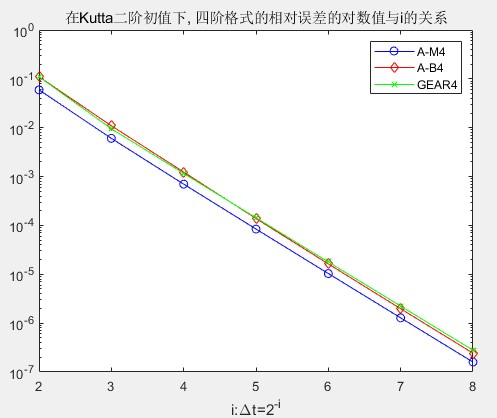
\includegraphics[width=0.7\textwidth]{6}
	\caption{Kutta二阶初值}
\end{figure}
\begin{figure}[H]
	\centering
	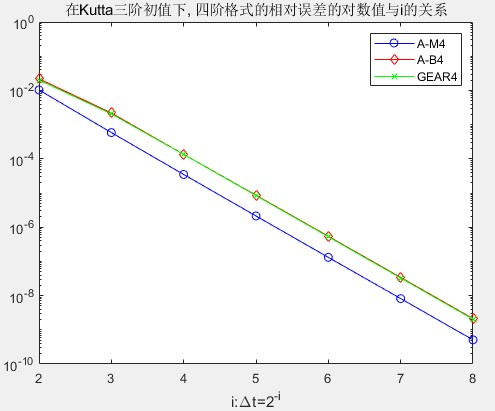
\includegraphics[width=0.7\textwidth]{7}
	\caption{Kutta三阶初值}
\end{figure}
\begin{figure}[H]
	\centering
	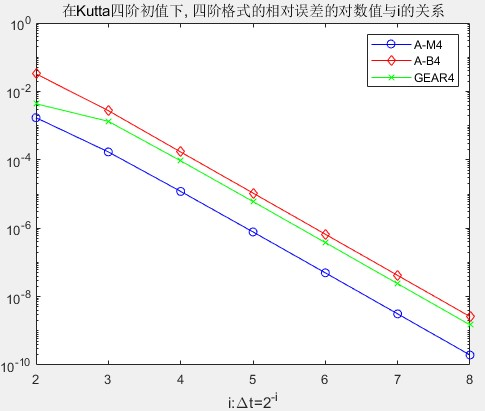
\includegraphics[width=0.7\textwidth]{8}
	\caption{Kutta四阶初值}
\end{figure}























%\underline{首先考虑精确初值下, 不同格式与精确解的绝对误差:}
%
%
%
%\noindent 当初值是精确时, 收敛性最差的是A-B四阶格式, 但其全局误差仍被控制在$6.7\times10^{-5}$以内; 其次是Gear四阶格式, 其绝对误差被控制在$3.6\times10^{-5}$以内; 此时最优越的是A-M四阶隐格式, 被控制在$5.26\times10^{-6}$以内.
%\begin{figure}[H]
%	\centering
%	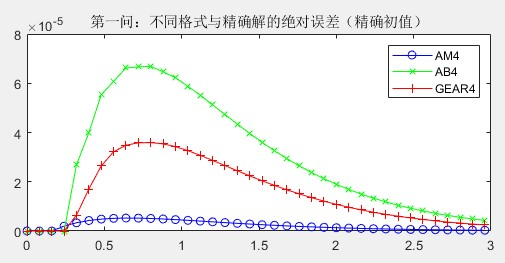
\includegraphics[width=1\textwidth]{精确初值不同格式}
%	\caption{精确初值不同格式与精确解的绝对误差}
%\end{figure}
%\quad \\
%\noindent \underline{考虑通过显式Euler格式求初值, 并计算不同格式与精确解的绝对误差:}\\
%发现通过显式Euler格式求出初值, 三个不同四阶格式与精确解的绝对误差相较于精确初值是糟糕的, 三者绝对误差只被控制在$3\times10^{-2}$以内, 这是因为显式Euler格式求出的初值与精确值相差大.记$u^{E}_i$是通过显式Euler格式求出的第$i$个近似值, 那么(以A-B四步四阶格式在显式Euler初值条件下求得的近似解的前$4$项为例)
%\begin{align*}
%	\vert u^{E}_1-u(t_1) \vert &\approx 1.21\times10^{-2}\\
%	\vert u^{E}_2-u(t_2) \vert &\approx 2.205\times10^{-2}\\
%	\vert u^{E}_3-u(t_3) \vert &\approx2.61\times10^{-2}
%\end{align*}
%\noindent 由于前三至四个初值具有一定的误差, 从而导致了三个不同格式的精度较差.
%
%
%\begin{figure}[H]
%	\centering
%	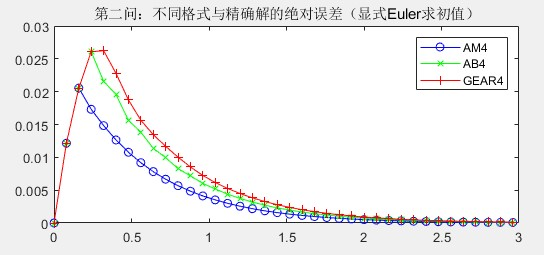
\includegraphics[width=1\textwidth]{Euler初值不同格式}
%	\caption{显Euler格式求得初值, 不同格式与精确解的绝对误差}
%\end{figure}
%\quad  \\
%\noindent \underline{再考虑通过Kutta二至四阶方法求解初值:}\\
%Kutta格式求解初值, 不同格式的精度较好: 通过Kutta二阶格式求得初值, 三个不同格式的绝对误差均被控制在$1.5\times10^{-3}$以内; 通过Kutta三至四阶格式求初值, 三个不同格式的绝对误差控制在$7\times10^{-5}$以内. 此外, A-M四阶格式在Kutta初值下的精度是最高的, 而Gear与A-B四阶格式的精度相当. 按照之前的方法考虑Kutta初值, 记$u^{Kj}_i$是Kutta的$j$阶格式求得的第$i$个近似值, 那么
%\begin{align*}
%	\vert u^{K2}_1-u(t_1) \vert &\approx 7\times10^{-4}\\
%	\vert u^{K2}_2-u(t_2) \vert &\approx 1.1\times10^{-3}\\
%	\vert u^{K2}_3-u(t_3) \vert &\approx 1.4\times10^{-3}
%\end{align*}
%\noindent 对比$\vert u^{K2}_i-u(t_i) \vert$与$\vert u^{E}_i-u(t_i)\vert$, 可以发现通过Kutta二阶格式求出的初值相较于通过显Euler格式求出的初值具有更高的精度. 且由于这是测试问题, 故也有$\vert f(t_i,u^{K2}_i)-f(t_i,u(t_i)) \vert=\vert a\vert \vert u^{K2}_i-u(t_i) \vert$以及$\vert f(t_i,u^{E}_i)-f(t_i,u(t_i)) \vert=\vert a\vert \vert u^{E}_i-u(t_i) \vert$, 从而由此导致精度的差别.
%\begin{figure}[H]
%	\centering
%	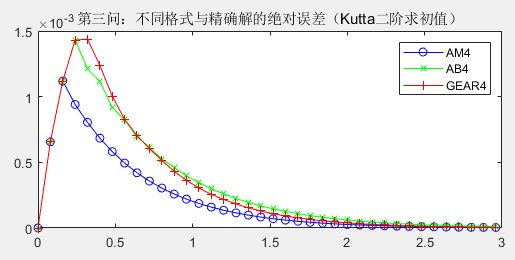
\includegraphics[width=1\textwidth]{K2初值不同格式}
%	\caption{Kutta二阶格式求得初值, 不同格式与精确解的绝对误差}
%\end{figure}
%\begin{figure}[H]
%	\centering
%	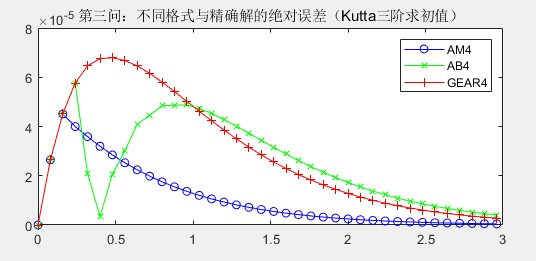
\includegraphics[width=1\textwidth]{K3初值不同格式}
%	\caption{Kutta三阶格式求得初值, 不同格式与精确解的绝对误差}
%\end{figure}
%\begin{figure}[H]
%	\centering
%	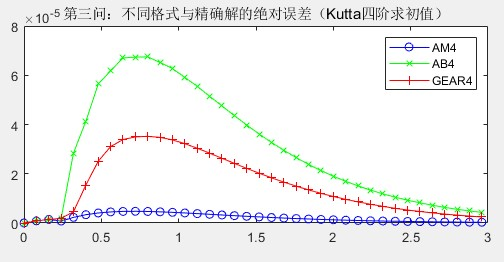
\includegraphics[width=1\textwidth]{K4初值不同格式}
%	\caption{Kutta四阶格式求得初值, 不同格式与精确解的绝对误差}
%\end{figure}
%\quad \\
%\noindent 通过五种不同方法(精确解、显式Euler、Kutta二至四阶)求解初值, 并在相同初值的条件下计算不同的四阶格式, 由上面的讨论发现当初值是由显式Euler格式求得时, A-M、A-B以及Gear四阶方法的精度相较于精确初值与Kutta二至四阶初值是具有较差的精度的, 从而在后续讨论中可以只考虑相同格式在精确初值与Kutta二至四阶初值之间对比.\\
%\quad \\
%\textbf{2) 不同的初值对相同格式的精度影响:}\\
%\noindent \underline{A-M四阶格式在不同初值条件的精度:}\\
%首先比较A-M四阶格式在精确初值、Kutta二至四阶初值条件下的表现: 可以发现Kutta二阶初值条件相较于其他三个初值条件, 它的精度较差. 为了进一步观察精度, 比较A-M四阶格式在精确初值、Kutta三至四阶初值条件的精度.
%\begin{figure}[H]
%	\centering
%	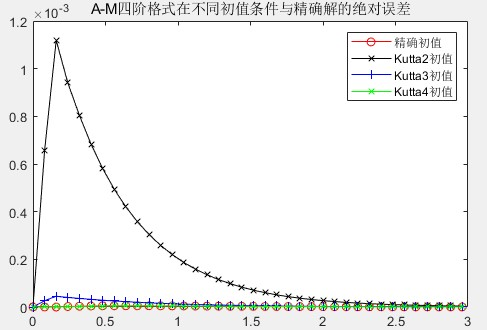
\includegraphics[width=0.83\textwidth]{AM4不同初值}
%	\caption{A-M四阶格式在不同初值条件下, 与精确解的绝对误差}
%\end{figure}
%\begin{figure}[H]
%	\centering
%	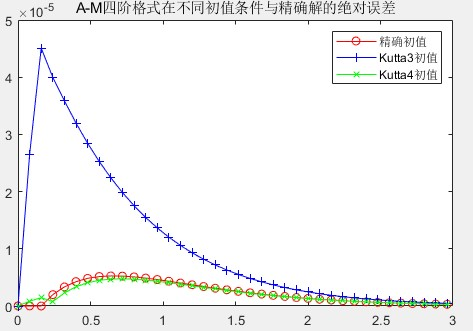
\includegraphics[width=0.83\textwidth]{AM4不同初值2}
%	\caption{A-M四阶格式在精确初值、Kutta三至四阶初值条件下, 与精确解的绝对误差}
%\end{figure}
%
%\noindent 在数值上有如下(记$u^p_i$是精确初值条件下的近似值第$i$项):
%\begin{align*}
%	\max_{1 \le i \le N} \vert u^{p}_i - u(t_i)\vert &\approx5.2\times10^{-6}\\
%	\max_{1 \le i \le N} \vert u^{E}_i - u(t_i)\vert &\approx2\times10^{-2}\\
%	\max_{1 \le i \le N} \vert u^{K2}_i - u(t_i)\vert &\approx1.1\times10^{-3}\\
%	\max_{1 \le i \le N} \vert u^{K3}_i - u(t_i)\vert &\approx4.5\times10^{-5}\\
%	\max_{1 \le i \le N} \vert u^{K4}_i - u(t_i)\vert &\approx4.75\times10^{-6}
%\end{align*}
%\noindent 从而得到了全局误差, 并可知当迭代格式是A-M三步四阶格式时, 显式Euler初值的精度时最差的, 二至三阶Kutta初值精度差于精确初值, 而Kutta四阶精度与精确初值的精度相当.\\
%
%\noindent \underline{A-B四阶格式在不同初值条件的精度:}
%\begin{figure}[H]
%	\centering
%	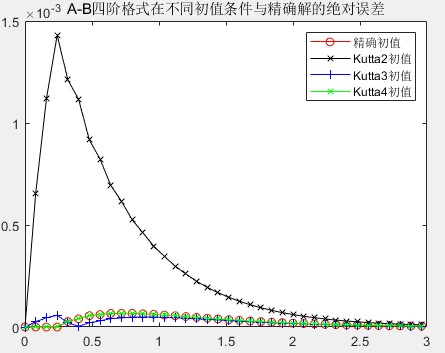
\includegraphics[width=0.8\textwidth]{AB4不同初值}
%	\caption{A-B四阶格式在不同初值条件下, 与精确解的绝对误差}
%\end{figure}
%\noindent 同样, 的Kutta二阶初值条件下的精度是较差的, 进一步考虑精确初值与三至四阶Kutta初值条件
%\begin{figure}[H]
%	\centering
%	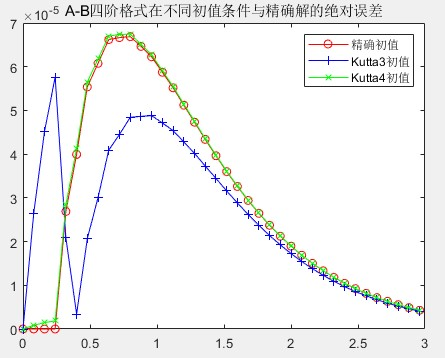
\includegraphics[width=0.8\textwidth]{AB4不同初值2}
%	\caption{A-B四阶格式在精确初值、Kutta三至四阶初值条件下, 与精确解的绝对误差}
%\end{figure}
%\noindent 由图9可知, 当格式为四步四阶A-B格式时, Kutta三阶初值条件下的精度反而要高于精确初值与Kutta四阶初值条件下的精度. 在数值上有以下:
%\begin{align*}
%	\max_{1 \le i \le N} \vert u^{p}_i - u(t_i)\vert &\approx6.7\times10^{-5}\\
%	\max_{1 \le i \le N} \vert u^{E}_i - u(t_i)\vert &\approx2.6\times10^{-2}\\
%	\max_{1 \le i \le N} \vert u^{K2}_i - u(t_i)\vert &\approx1.4\times10^{-3}\\
%	\max_{1 \le i \le N} \vert u^{K3}_i - u(t_i)\vert &\approx5.7\times10^{-5}\\
%	\max_{1 \le i \le N} \vert u^{K4}_i - u(t_i)\vert &\approx6.7\times10^{-5}
%\end{align*}
%\noindent 上面为A-B四阶格式在不同初值条件下的全局误差, 其中显式Euler格式初值条件下的精度最差; 其次是Kutta二阶初值条件下的精度; 而精确初值与三至四阶Kutta初值下的精度相当, 其中Kutta三阶初值条件反而更优越.\\
%
%\noindent \underline{Gear四阶格式在不同初值条件的精度:}\\
%类似于上面讨论, 全局误差有以下估计
%\begin{align*}
%	\max_{1 \le i \le N} \vert u^{p}_i - u(t_i)\vert &\approx3.6\times10^{-5}\\
%	\max_{1 \le i \le N} \vert u^{E}_i - u(t_i)\vert &\approx2.6\times10^{-2}\\
%	\max_{1 \le i \le N} \vert u^{K2}_i - u(t_i)\vert &\approx1.4\times10^{-3}\\
%	\max_{1 \le i \le N} \vert u^{K3}_i - u(t_i)\vert &\approx6.8\times10^{-5}\\
%	\max_{1 \le i \le N} \vert u^{K4}_i - u(t_i)\vert &\approx3.5\times10^{-5}
%\end{align*}
%\begin{figure}[H]
%	\centering
%	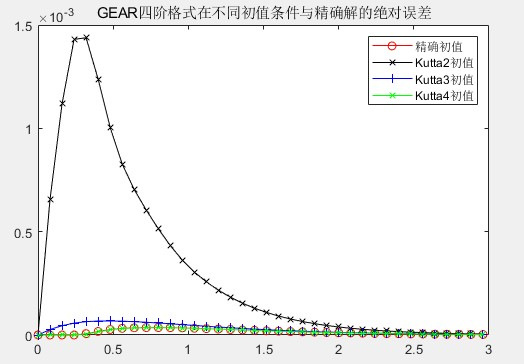
\includegraphics[width=0.8\textwidth]{GEAR4不同初值}
%	\caption{Gear四阶格式在不同初值条件下, 与精确解的绝对误差}
%\end{figure}
%\noindent 同样, 的Kutta二阶初值条件下的精度是较差的, 进一步考虑精确初值与三至四阶Kutta初值条件
%\begin{figure}[H]
%	\centering
%	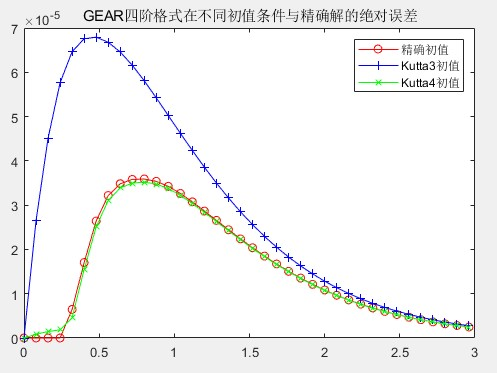
\includegraphics[width=0.8\textwidth]{GEAR4不同初值2}
%	\caption{Gear四阶格式在精确初值、Kutta三至四阶初值条件下, 与精确解的绝对误差}
%\end{figure}
%
%\noindent 从而由以上可知, 当格式为Gear四阶格式时, 在显式Euler格式初值条件下的精度时最差的; 其次为Kutta二阶初值条件下的精度; 然后精确初值、Kutta三至四阶初值条件下的精度量级相当, 其中Kutta三阶初值下的精度稍次于另外两个初值条件下的精度.

	
\end{document}